\documentclass[12pt]{article}

\usepackage{setspace}
\usepackage{minted}
\usepackage{fancyvrb}
\usepackage{listings}
\usepackage{graphicx}

\usepackage[margin=0.75in]{geometry}
\pagestyle{empty}

\def \name       {Enrique Gavidia}
\def \coursenum  {CSC 415.01}
\def \coursename {Operating Systems Principles}
\def \instructor {Prof. Murphy}
\def \semester   {Spring 2012}
\def \assignment {Homework \# 6}
\def \duedate    {April 27, 2012}

\newcommand {\mytilde} {$\sim$}
\newcommand {\comment}[1] {\textcolor{red}{#1}}
\newcommand {\filename}[1] {\flushleft \textbf{#1}}
\newcommand {\append}[2] {\section*{Appendix #1} \textsl{\large #2}}

\newcommand {\makecover} {
  \begin{titlepage}
    \begin{center}
      \LARGE{\coursenum, \semester \\ \coursename}\\
      \Large{\instructor}\\
      \vfill
      \textbf{\Huge \assignment}\\
      \vfill
      \Large{\name}\\
      \large{\duedate}
    \end{center}
  \end{titlepage}
}

\DefineVerbatimEnvironment {shelloutput} {Verbatim} {fontsize=\scriptsize, numbers=left, frame=lines, commandchars=\%\{\}}

\newcommand {\includesource}[2] {\inputminted[linenos, fontsize=\scriptsize, frame=lines]{#1}{#2}}
\newcommand {\includeoutput}[1] {\VerbatimInput[fontsize=\scriptsize, numbers=left, frame=lines, commandchars=\%\{\}]{#1}}

\begin{document}

\makecover

%---{ Main Content }--------------------------------------------------------------------
\section*{Assignment Description}
For this assignment, we were to explore concurrency+parallelism using single and multiple core environments, through the monitoring 
of performance when running concurrent programs. Our task was to implement a multi-threaded searching algorithm that partitions a
large data set into a specified number of chunks, and searches them concurrently for a search key.  We then had to measure the performance
of the algorithm in both Windows and Unix environments with Single and Multiple CPU cores.  The focus of the monitoring was to compare
the advantages of running concurrent code in a parallel multi-core environment, as opposed to a single-core environment. To aid in this
comparison, we graphed the performances of all the different systems as functions of the program's number of threads, versus the time
they took to complete. The results supported the notion that multiple parallel processor systems are more efficient at executing concurrent 
code than single core systems.

 
This code has been tested to work under \textsl{Windows}, \textsl{Gentoo Linux}, and \textsl{Mac OSX}.
The implementation for \textsl{Unix} is under \textbf{Appendix II}, and the \textsl{Windows} implementation is in \textbf{Appendix IV}. 
The \textsl{Pseudocode} outlining the design of both implementations is in \textbf{Appendix I}.
And the graphs for the outputs of the different systems are located under \textbf{Appendix VI}.


\section*{Design \& Implementation}
The design of the program is fairly simple and straightforward; I wrote the implementations just as they ere outlined in the Pseudocode.
The threads each search a separate partition of the data set, and store their results in another array, which is then searched for
errors as it is being output to the user. In Unix there wasn't much trouble getting the algorithm to run and yield it's performance 
results as expected, but for the Windows implementation however, there wasn't a straightforward way to truly accurately measure time in 
microseconds with the Win32 API for the performance measurement portion of the assignment. Instead, the API provides access to the CPU's 
internal clock counter, which is what I used to then extrapolate a simple approximation of the algorithm's elapsed time in microseconds.  
Another obstacle with the Windows implementation was the limited range of the platform's \texttt{rand()} function, which is prone to causing 
many 'error' results with duplicate keys at the array sizes we were dealing with. The array's size of $2^{18}$ was roughly an order of magnitude 
larger than the largest value produced by the \texttt{rand()} function, so in order to minimize the possibility of errors while still maintaining 
a reasonable chance for the array to contain the search key, I multiplied the results of two calls to \texttt{rand()} together, and restricted 
their domain to twice the size of the array; i.e. 2($2^{18}$).


\section*{Results}
As for the results of the performance tests, the single-core systems performed as expected, handling the algorithm with 1 thread better than with multiple threads, but the Windows single-core machine seemed to have experienced a noticeably higher spike when attempting to run 4 or more threads. Both of the multi-core tests were performed on Dual-core systems, and both performed about the same in handling multiple threads better than the single-core system.


\section*{Improvements}
I would probably simply improve this algorithm by switching it to use linked-lists instead of arrays, so that it can make better use of a system's memory and allow for larger sets of data,
since linked-lists do not require the system to have large contiguous pools of memory available for usage like arrays do. This should consequently also help the algorithm's performance
on systems with low memory.


%---{ Appendices }-----------------------------------------------------------------------
%\newpage

%----{ Unix }--------------------------------------------------------------------------

\append{I} {Pseudocode}
\begin{scriptsize}
\begin{verbatim}
int threads[];
int array[];
int search_results[];
int search_key;

semaphore sem;

search_array() {
    // search array for search key
    P(sem);
}

main() {

    // initialize random array and search key

    initialize_semaphore(s);

    for (thread in threads) {
        start_thread(thread, search_array)
    }

    for (thread in threads) {
        V(sem);
        end_thread(thread);
    }

    // check for 'errors'
    int errors = 0;
    for (result in search_results) {
        if (result != -1 && key already found)
            errors++;
    }
}
\end{verbatim}
\end{scriptsize}


\append{II} {Unix Source Code}
\includesource{c}{unix_search.c}

\append{III} {Unix Output}
\filename{Single-core}
\includeoutput{output/unix_search_singlecore.txt}

\filename{Multi-core}
\includeoutput{output/unix_search_multicore.txt}

%----{ Windows }--------------------------------------------------------------------------
\append{IV} {Windows Source Code}
\includesource{c}{win_search.c}

\append{V} {Windows Output}
\filename{Single-core}
\includeoutput{output/win_search_singlecore.txt}

\filename{Multi-core}
\includeoutput{output/win_search_multicore.txt}

\append{VI} {Graphs}
% Time (Y) vs # of Threads (x)


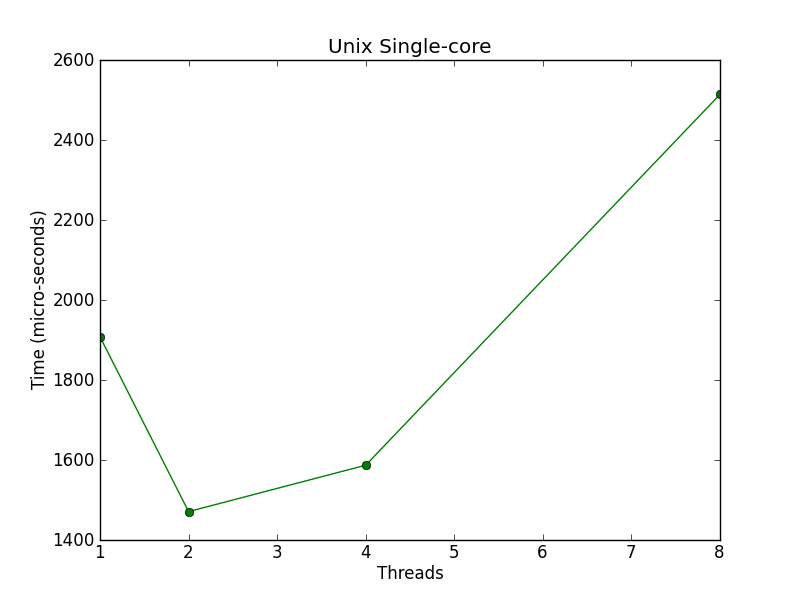
\includegraphics[scale=0.4]{output/unix_singlecore_graph.png} 
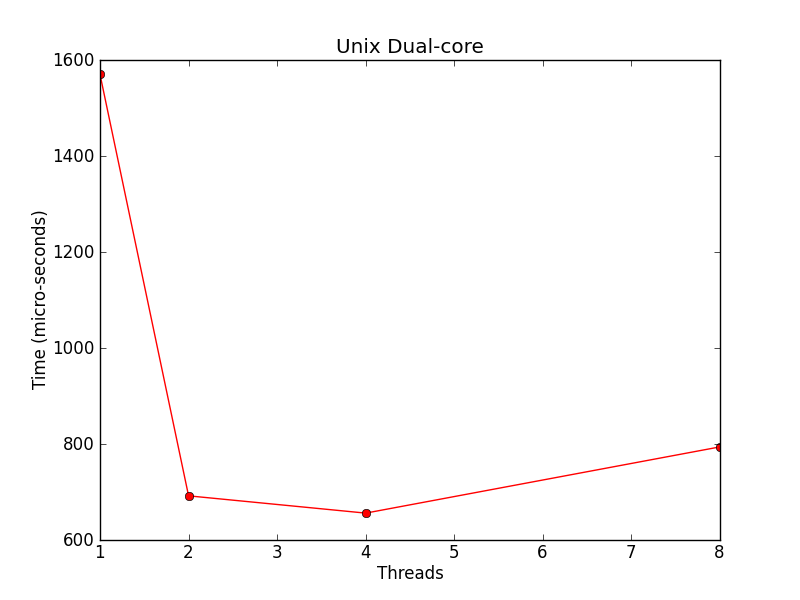
\includegraphics[scale=0.4]{output/unix_multicore_graph.png}
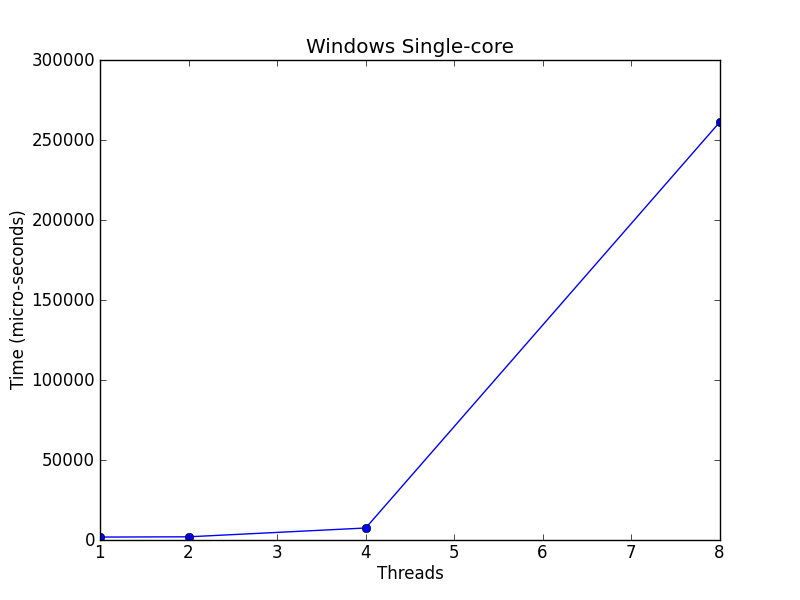
\includegraphics[scale=0.4]{output/win_singlecore_graph.png} 
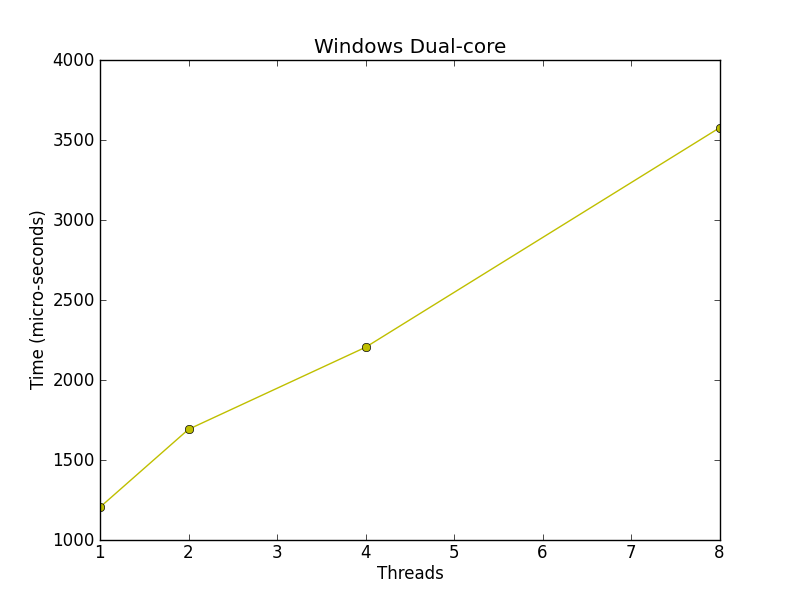
\includegraphics[scale=0.4]{output/win_multicore_graph.png}


\end{document}
